\section{\acl{LSTM}}

\subsection{Einleitung}
\ac{LSTM} ist ein \ac{RNN}, welches die Eigenschaft hat Zustände über einen
bestimmten Zeitraum zu behalten und danach wieder zu vergessen. \acp{LSTM} sind
somit eine spezielle Form von \acp{MLP}. Ein \ac{LSTM} definiert rekurrente
Verbindungen (Verbindungen von Neuronen zu vorhergehenden bzw. denselben
Neuronen) in der Art und Weise, dass die Eingabe Daten bzw.
die Ausgabe Daten gespeichert über mehrere Aufrufe des Netzwerkes hinaus
gespeichert werden. Diese gespeicherten Daten werden bei bestimmten
Eingangsdaten Ausgegeben, bei anderen \textit{vergessen} bzw. überschrieben oder
nicht verwendet. 
 
\acp{RNN} und vielmehr noch \acp{LSTM} sind Modelle für das menschliche Gehirn.
Im Gehirn sind viele Neuronen untereinander, also mit sich selbst, nachfolgenden
und vorhergehenden Nueronen vernetzt, sogenannten Feedback Verbindungen. Jedes
Neueron ist dabei ein speziell aufgebaut um Informationen zu speichern.
\acp{RNN} haben keine bzw. einfache Erinnerungsneuronen und sind aus diesem
Grund nicht für länger Erinnerungen geeignet. Bei \acp{LSTM} hingegen sind
komplexe Erinnerungsneuronen (\ac{LSTM}-Neuronen) miteinander verknüpft. Jedes
einzelne Neuron kann Informationen über einen längeren Zeitraum, d.h. auch bei
häufiger Nutzung des Netzes, Daten speichern. Dadurch dass \acp{LSTM} Daten auch
nach dem Training speichern können, also verschiedene Zustände haben,
unterscheiden sie sich von vielen anderen Machine Learning Verfahren, wie z.B.
\ac{HMM} oder \acp{SVM}. Sie sind besonders für komplexe Aufgaben mit unscharfen
Beobachtungen geeignet und werden bevorzugt in Handschrift- und Spracherkennung,
Proteinanalyse und weiteren dynamischen Feldern verwendet. Durch die Analogie
zum Gehirn können \acp{LSTM} biologisch motiviert werden.
 
\subsection{Architektur von \aclp{LSTM}}
Ein \ac{RNN} mit \ac{LSTM} Einheiten hat ein Hiddenlayer in dem die
verschiedenen \ac{LSTM} Knoten enthalten sind. Das Outputlayer ist dann ein
einfaches lineares oder sigmoidales Layer.  
\begin{figure}[h]
	\begin{center}
	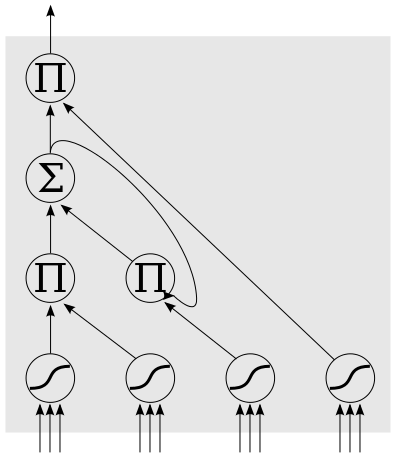
\includegraphics[scale=0.5]{lstm_block}
	\caption{Schema eines \acs{LSTM} Blocks}
	Quelle: \cite{WIKI2013}
	\label{fig:lstm_block}
	\end{center}
\end{figure}


\subsection{Funktionsweise von der \acs{PyBrain} \acs{LSTM} Implementierung}
\ac{PyBrain}\cite{schaul2010} ist eine Bibliothek für Python und stellt
verschiedene Module aus dem Bereich des maschinellen Lernes bereit. Dabei
spielen neuronale Netzwerke eine zentrale Rolle, diese werden in verschiedenen
Lernmethoden angewendet wie z.B. im Reinforcement, unüberwachten oder
evolutionären Lernen.

\begin{lstlisting}[caption={Aufbau eines LSTM Netzes},label={lst:lstm_example}]{lst:lstm_example} 
net = buildNetwork(INPUTS, HIDDEN, OUTPUTS, hiddenclass=LSTMLayer,
outclass=SigmoidLayer, recurrent=True, bias=True) 
ds = DATASET trainer = BackpropTrainer(net, ds)
for _ in range(1000):
    trainer.train()
\end{lstlisting}
 
In \autoref{lst:lstm_example} ist ein Beispiel aufgezeigt wie
\ac{PyBrain} verwendet werden kann. Es gibt dabei verschiedene Möglichkeiten im Aufbau des Netzes
(v.a. Anzahl der Neuronen und \ac{LSTM}-Blocks), in der Datenhaltung
(\ref{sec:lstm_data}) sowie in der Trainingsmethode (z.B. Backpropagation). 
Die \ac{PyBrain} Implmenetierung bringt bereits die Umsetzung der
\ac{LSTM}-Blocks mit, sodass die konkrete Umsetzung der Blöcke nicht
durchgeführt werden muss. 

\subsection{Verwendetes Datenmodell}
\label{sec:lstm_data}

Im \autoref{sec:gestures_dataformat} wird beschrieben wie Gesten aufgenommen und
abgespeichert werden. Dabei wird ein Trainingsdatenset erzeugt, dass für
jeden Datensatz eine bestimmte Anzahl an Frames mit je 64 Datenpunkte im
gewünschteen Frequenzbereich enthält. 

Für das \ac{LSTM} Netz wird jeder Datensatz als linear aus den einzelnen Frames
aufgebaut. Dadurch entsteht ein einzelner Eingabevektor inkl. der
Klassifizierung. Zur Vereinheitlichung werden die Daten noch normalisiert. Dies
ist notwendig, da Datensätze unter verschiedenen Bedingungen erzeugt werden
können, z.B. im lauten Umfeld, andere Anordnung von Mikrofon und Lautsprecher,
unterschiedlicher Größe der Hände, unterschiedliche Lautstärke, etc. Um
vergleichbare Daten zu erhalten wird daher die Amplitude der Referenzfrequenz
als Normailisrungsfaktor verwendet, diese ist i.d.R. am größten. Durch diese
Normalisierung Referenzfrequenz auf 1 werden alle weiteren Datenpunkte im
Intervall zwischen 0 und 1 liegen. 

Zur Unterscheidung von Gesten zum Hintegrundrauschen kann noch ein Datenset mit
Hintergreundrauschen genutzt werden. Hier muss sich noch zeigen wie gut das
\ac{LSTM} Netz ohne diese Daten klassifiziert, je nach Ergebnis wird es noch
hinzugezogen. 





\nocite{GERS2001,WIKI2013,Schmidhuber2013,LSTM1,Nerbonne1}
